% cd "/Users/pluttan/Desktop/_Сем1/BMSTU-1/ОП/Подготовка к экзамену/"&&cp -r "/Users/pluttan/Desktop/_Сем1/BMSTU-1/ОП/Подготовка к экзамену/"img/ "/Users/pluttan/Desktop/_Сем1/BMSTU-1/ОП/Подготовка к экзамену/"conf/&&cp "/Users/pluttan/Desktop/_Сем1/BMSTU-1/ОП/Подготовка к экзамену/"examOP.tex "/Users/pluttan/Desktop/_Сем1/BMSTU-1/ОП/Подготовка к экзамену/"conf/&&cd "/Users/pluttan/Desktop/_Сем1/BMSTU-1/ОП/Подготовка к экзамену/"conf/&&/usr/local/texlive/2022/bin/universal-darwin/xelatex --shell-escape examOP.tex&&cp "/Users/pluttan/Desktop/_Сем1/BMSTU-1/ОП/Подготовка к экзамену/"/conf/examOP.pdf "/Users/pluttan/Desktop/_Сем1/BMSTU-1/ОП/Подготовка к экзамену/"/

\documentclass[a4paper, 10pt]{article}
\usepackage[T2A]{fontenc}
\usepackage[left=2cm,right=2cm,top=2cm,bottom=2cm]{geometry}
\usepackage[russian]{babel}
\usepackage{amsfonts,amsmath,amssymb}
\usepackage{mathrsfs}
\usepackage{graphicx}
\usepackage[normalem]{ulem}
\usepackage{wrapfig}
\usepackage{fancyhdr}
\usepackage{floatflt}
\usepackage{python}
\usepackage{float}
\usepackage{ amssymb }
\usepackage{indentfirst}
\usepackage{setspace}
\usepackage{scrextend}
\usepackage{listings}
\usepackage{makecell,tabularx}
\usepackage{hyperref}
\usepackage{xcolor}

\newcommand{\rub}{{\rm{Р}\kern-.635em\rule[.5ex]{.52em}{.04em}\kern.11em}}

\definecolor{linkcolor}{HTML}{000000} 
\definecolor{urlcolor}{HTML}{0000FF} 

\hypersetup{pdfstartview=FitH,  linkcolor=linkcolor,urlcolor=urlcolor, colorlinks=true}

\definecolor{grey}{RGB}{40, 40, 40}

\renewcommand{\href}[1]{\url{#1}}

\lstdefinestyle{CommentStyle}{
    language=XML,
    %numbers=left, numberstyle=\tiny, stepnumber=1, numbersep=5pt,
    commentstyle=\color{red},
	basicstyle=\footnotesize\ttfamily,
	language={[ANSI]C++},
	keywordstyle=\bfseries,
	showstringspaces=false,
	morekeywords={include, printf},
	commentstyle={},
	escapeinside=§§,
	escapebegin=\begin{russian}\commentfont,
	escapeend=\end{russian},
    keywordstyle=\color{blue}\bfseries,
    morekeywords={align,begin},
    extendedchars=\true,
    tabsize=2
}
\lstdefinestyle{myLatexStyle}{
    language=c++,
    %backgroundcolor=\color{grey},
    numbers=left, numberstyle=\tiny, stepnumber=1, numbersep=5pt,
    commentstyle=\color{red},
    keywordstyle=\color{blue}\bfseries,
    morekeywords={align,begin},
    extendedchars=\true,
    tabsize=2
}

\lstdefinestyle{pmyLatexStyle}{
    language=java,
    %backgroundcolor=\color{grey},
    numbers=left, numberstyle=\tiny, stepnumber=1, numbersep=5pt,
    commentstyle=\color{red},
    keywordstyle=\color{blue}\bfseries,
    morekeywords={align,begin},
    extendedchars=\true,
    tabsize=2
}

\setlength{\parindent}{12,5mm}

\newcommand{\bvec}[1]{\overrightarrow{#1}}
\newcommand{\mcol}[1]{\multicolumn{2}{c}{#1}}
\newcommand{\mcolt}[1]{&#1&}
\renewcommand{\a}{\vec{a}}
\renewcommand{\b}{\vec{b}}
\renewcommand{\c}{\vec{c}}
\renewcommand{\d}{\vec{d}}
\renewcommand{\i}{\vec{i}}
\renewcommand{\j}{\vec{j}}
\renewcommand{\k}{\vec{k}}
\newcommand{\nul}{\vec{0}}

\newcommand{\logo}{\vcenter{\hbox{\includegraphics[width=.8em]{/Users/pluttan/Documents/bw2.png}}}}
\onehalfspacing

\pagestyle{fancy}
\renewcommand{\sectionmark}[1]{\markright{#1}}
\fancyhf{} 
\fancyhead[R]{\bfseries\thepage}
\fancyhead[LO]{$\mathfrak{Copyright}\ \mathfrak{pluttan} \logo$}

\newcommand{\image}[2]{
	\begin{figure}[H]
		\center{\includegraphics[height=#2pt]{img/#1} }
    \end{figure}
}

\newcommand{\dotitle}[3]{

\thispagestyle{empty}
\sloppy{
  \scriptsize{
    \line(6,0){0}

    \centering $\mathfrak{Copyright}\ \mathfrak{pluttan} \logo$

    \centering Привет! Меня зовут Андрей, я создаю свою ботву, этот файл малая ее часть. 
    
    \centering Пользоваться и распространять файлы конечно же можно. Если вы нашли ошибку в файле, можете 
    
    \centering исправить ее в исходном коде и подать на слияние или просто написать в issue. 
    
    \centering Приятного бота)

    \line(6,0){300}

    \centering GitHub: https://github.com/pluttan

    \line(6,0){0}
  }}

\topskip=-200pt
\vspace*{130pt}
\begin{Huge}
  \textbf{
    \begin{center}
        #1
    \end{center}
  }
  {\begin{center} 
        #2
    \end{center}}
\end{Huge}
\vspace*{300pt}
  \begin{flushright}
    Над файлом работали: \\
    pluttan\\
    #3
  \end{flushright}
\newpage
\pagestyle{fancy}
\renewcommand{\sectionmark}[1]{\markright{#1}}
\fancyhf{} 
\fancyhead[R]{\bfseries\thepage}
\fancyhead[LO]{$\mathfrak{Copyright}\ \mathfrak{pluttan} \logo$}
}


% It's XeLaTeX, if you can't compile comment this line 
\usepackage{fontspec}\setmainfont{Times New Roman} 

\include{/Users/pluttan/Documents/forMyDocs/preambMisha.tex}
\newcommand{\hbook}[1]{{\small\begin{center}\textit{Иванова Г.С. Основы программирования 2002, стр. #1}\end{center}}}
\newcommand{\hprez}[2]{{\small\begin{center}\textit{Иванова Г.С. Курс Основы программирования, през. #1, сл. #2}\end{center}}}



\begin{document}
\tikz[remember picture,overlay] \node[opacity=0.1,inner sep=0pt] at (current page.center){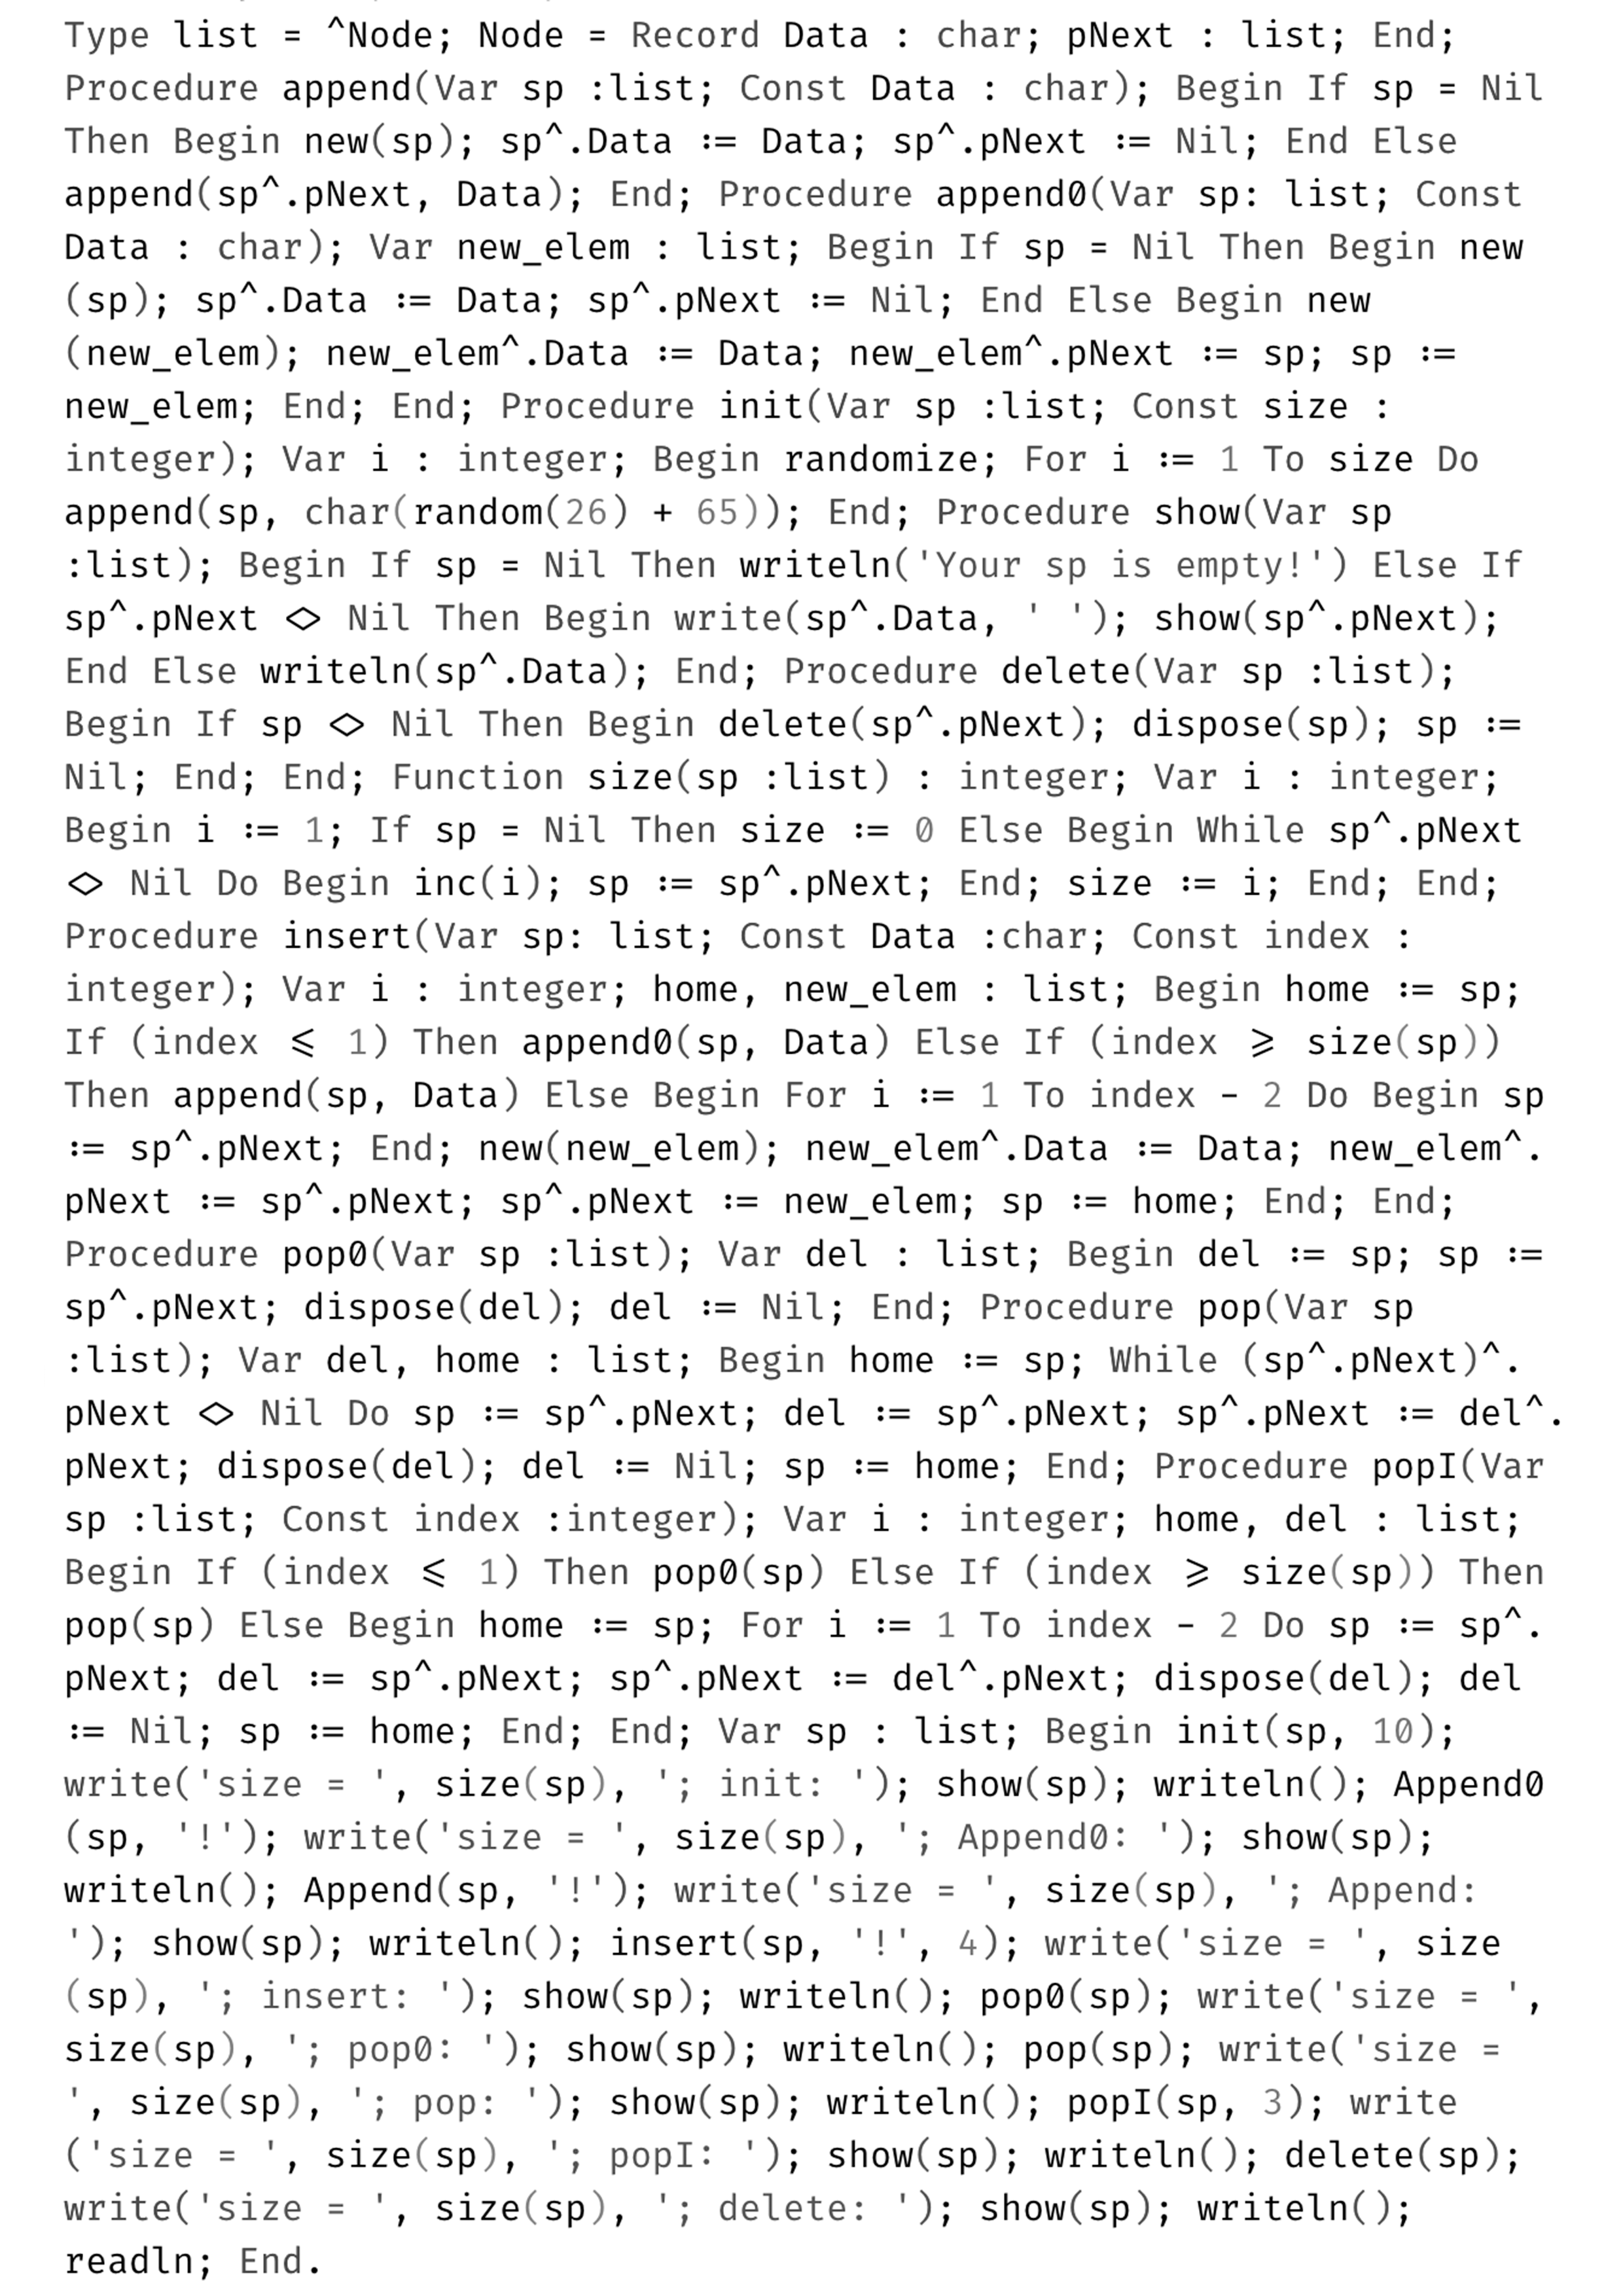
\includegraphics[width=\paperwidth,height=\paperheight]{../img/bg1.png}};
\dotitle{Подготовка к экзамену}{Основы программирования}
\toc

\section{Теоритическая часть}

%================================
%          Вопрос 1
%================================

\subsection{Синтаксис  и  семантика  языков  программирования.  Алфавит  языка  Pascal.  Описание синтаксиса языка: синтаксические диаграммы. Примеры. }

\begin{myquote}
\hbook{28 - 30}

\hprez{1}{9, 26}
\end{myquote}
\large

{\bf{Синтаксис}}
 - совокупность правил, определяющих допустимые конструкции (слова, предложения) языка, его форму. «Защищенный» синтаксис предполагает, что предложения языка строятся по правилам, которые позволяют автоматически выявлять большой процент ошибок в программах.

{\bf{Семантика}}
 - совокупность правил, определяющих смысл синтаксически корректных конструкций языка, его содержание. Ясная или «интуитивно-понятная» семантика – семантика, позволяющая без большого труда определять смысл программы или «читать» ее.

\noindent
{\bf{Алфавит языка Паскаль  }}

\begin{enumerate}
\item Латинские буквы без различия строчных и прописных;
\item Арабские цифры: \texttt{0, 1, 2, 3, 4, 5, 6, 7, 8, 9};
\item Шестнадцатеричные цифры: \texttt{0..9, a..f} или \texttt{A..F};
\item Специальные символы: \texttt{+ - * / = := ; }и т. д.;
\item Служебные слова: \texttt{do, while, begin, end} и т. д.
\end{enumerate}

{\bf{Описание синтаксиса языка}}
включает определение алфавита и правил построения различных конструкций языка из символов алфавита и более простых конструкций. Для этого обычно используют синтаксические диаграммы.

{\bf{Синтаксические диаграммы}}
отображают правила построения конструкций в более наглядной форме.
На такой диаграмме:
\begin{itemize}
\item символы алфавита изображают блоками в овальных рамках;
\item названия конструкций в прямоугольных рамках;
\item правила построения конструкций – в виде линии со стрелками на концах;
\item разветвление линии означает, что при построении конструкции есть варианты. 
\end{itemize}
% TODO: caption
% Пример: синтаксическая диаграмма, иллюстрирующая первые два правила описания конструкции <целое>
Синтаксическая диаграмма конструкции <целое>:
\image{exm1.png}{100}

%================================
%          Вопрос 2
%================================

\newpage\subsection{Представление  данных  в  языке  Pascal:  константы  и  переменные.  Классификация  скалярных типов данных, их внутреннее представление, операции над ними. Примеры.} 

\begin{myquote}
\hbook{31 - 40}

\hprez{1}{27 - 43}
\end{myquote}

{\bf{Константы}} – определяются один раз и не изменяются во время выполнения программы.
Используют следующие типы констант:
\begin{enumerate}
    \item Целые и вещественные десятичные числа;
    \item Шестнадцатеричные числа;
    \item Логические константы;
    \item Символьные константы – (записываются либо в апострофах, либо в виде соответствующих кодов по таблице ASCII);
    \item Строки символов – записываются в апострофах;
    \item Конструкторы множеств;
    \item Нулевой адрес – \texttt{nil}.
\end{enumerate}

\noindent
Константы используются в двух формах: 
\begin{itemize}
    \item {\bf{Литерал}} – представляет собой значение константы, записанное непосредственно в программе;
    \item {\bf{Поименованные константы}} объявляются в инструкции раздела описаний \texttt{const}. Обращение к ним осуществляется по имени (идентификатору).
\end{itemize}
\image{exm3.jpg}{90}

{\bf{Переменные}} – поименованные значения, которые могут изменяться в процессе выполнения программы. Их объявление выполняют в разделе описаний программы, причем указывается не только идентификатор переменной, но и ее тип. Обращение к переменным также осуществляют по идентификатору.

{\bf{Тип переменной}} – определяет возможный набор значений данной переменной, размер ее внутреннего представления и множество операций, которые могут выполняться над переменной.

\image{exm4.jpg}{110}

{\bf Простые (скалярные) типы} описывают упорядоченные наборы значений. Они делятся на {\bf порядковые} и {\bf вещественные}.



\image{exm5.jpg}{300}

\begin{itemize}
\item {\bf {Группа порядковых типов}} объединяет типы переменных, набор значений которых конечен.

    \begin{itemize}    
    \item {\bf{Стандартные типы}}

        {\small
        \begin{center}
        \begin{tabular}{ | c | c | c | c | }
        \hline
        Название & Обозначение & Диапазон значений & Длина внутреннего представления, байт\\
        \hline
        Целое & \texttt{Integer} & -32768..32767 & 2 (со знаком) \\
        \hline
        Короткое целое & \texttt{ShortInt} & -128..127 & 1 (со знаком) \\
        \hline
        Длинное целое & \texttt{LongInt} & $-2^{31}$..$2^{31}$ -1 & 4 (со знаком) \\
        \hline
        Байт & \texttt{Byte} & 0..255 & 1 (без знака) \\
        \hline
        Слово & \texttt{Word} & 0..65535 & 2 (без знака) \\
        \hline
        Логический & \texttt{Boolean} & \texttt{True, false} & 1 \\ 
        \hline
        Символьный & \texttt{Char} & Символы по таблице ASCII & 1\\
        \hline
        \end{tabular}
        \end{center}
        }
        
        \begin{itemize}
            \item {\bf{Логический тип}} \texttt{Boolean} включает два значения – \texttt{true(1)} и \texttt{false(0)}, но в памяти значения данного типа занимают целый байт;

            \item {\bf{Символьный тип}} \texttt{char} определяет набор символов по таблице ASCII. 
        \end{itemize}

    \item {\bf{Перечисляемый тип (перечисление)}} 
        – формируется из значений, определенных программистом при объявлении типа. Перечень задают через запятую в круглых скобках. Во внутреннем представлении значения перечисляемого типа кодируются целыми числами, начиная с нуля. Например:


    \texttt{Var D : (Mon, The, Wed, Thu, Fri, Sat, Sun);}  \{переменная D принимает одно из перечисленных значений\}

    \texttt{Mon = 0; The = 1 ... Sun = 6;}


    \item {\bf{Отрезок}}
        – определяется как диапазон значений некоторого уже определенного типа. Например: 

    \texttt{Var D : 1..31;}

    \end{itemize} 

    \item {\bf {Группа вещественных типов}} объединяет типы с условно бесконечным набором значений.
    {\small
    \begin{center}
        \begin{tabular}{ | c | c | c | c | c | }
        \hline
    Название & Обозначение & Кол-во десятичных  & Диапазон изменения  & Длина внутреннего \\
    &&значащих цифр&порядка&представления, байт\\
        \hline
        Вещественный & \texttt{Real} & 11..12 & -39..+38 & 6\\
        \hline
        Одинарной точности & \texttt{Single} & 7..8 & -45..+38 & 4\\
        \hline
        Двойной точности & \texttt{Double} & 15..16 & -324..+308 & 8\\
        \hline
        Расширенный & \texttt{Extended} & 19..20 & -4951..4932 & 10\\
        \hline
        Большое целое & \texttt{Comp} & 19..20 & $-2^{63}+1.. 2^{63}-1$ & 8 \\
        \hline
        \end{tabular}
    \end{center}
    }
\end{itemize}
\vspace*{10pt}
\noindent
{\bf{Операции}}
\begin{enumerate}

\item {\bf{Арифметические операции}} – применяют к вещественным и целым константам и переменным:
\texttt{+,  -, *, }

\texttt{/}  - \{вещественное деление\},

\texttt{div}  - \{целочисленное деление\}, 

\texttt{mod } - \{остаток от деления\}

*приоритет операций рассчитывается как в математике (+ скобки).

\image{exm6.jpg}{60}

\item {\bf{Операции отношения (больше, меньше, равно и т.д.)}} – применяют к числам, символам, строкам – в результате получают логическое значение: \texttt{<, >, =}, \texttt{<>} \{не равно\}, \texttt{<=} \{меньше или равно\}, \texttt{>=} \{больше или равно\}

% \texttt{<} \{меньше\}, \texttt{>} \{больше\}, \texttt{=} \{равно\}, 


\item {\bf{Логические операции}} – применяют к логическим значениям – результат логическое значение: \texttt{not, and, or, xor}

\item {\bf{Поразрядные операции}} – выполняются поразрядно, применяют к целым, результат – целое число: \texttt{not, and, or, xor, shr } - \{сдвиг вправо\}, \texttt{shl}  - \{сдвиг влево\} 
\end{enumerate}


%================================
%          Вопрос 3
%================================

\newpage\subsection{Совместимость типов данных и операции преобразования типов. Примеры. }

\begin{myquote}
\hbook{41 - 42}
    
\hprez{1}{43, 45}
\end{myquote}

\noindent
По правилам {\bf{совместимы}}:
\begin{enumerate}
    \item все целые типы между собой;
    \item все вещественные типы между собой;
    \item отрезок базового типа и базовый тип;
    \item два отрезка одного и того же базового типа;
    \item символ и строка.
\end{enumerate}

Для несовместимых типов результата и переменной, в которую его необходимо занести, при выполнении присваивания необходимо \textbf{явное преобразование типов}, например, посредством специальных функций:
\begin{itemize}
\item \texttt{trunc}(<Вещественное выражение>) – преобразует вещественное число в целое, отбрасывая дробную часть.

\item \texttt{round}(<Вещественное выражение>) – округляет вещественное число до целого по правилам арифметики.

Пример:   \texttt{trunc(4.5) = 4,    round(4.5) = 5 }

\item \texttt{ord}(<Порядковое выр.>) – преобразует значение в его номер.
Пример:   \texttt{ord(’A’)  = 65}.

\item \texttt{chr}(<Ц. выр.>) – преобразует номер символа в символ.
Пример:   \texttt{chr(65) = ’A’}.
\end{itemize}
\lstinputlisting[language=Pascal]{../Examples/b3_1.pas}


%================================
%          Вопрос 4
%================================

\newpage\subsection{Присваивание, условный оператор, оператор выбора. Синтаксис операторов, их особенности и примеры использования. }

\begin{myquote}
\hbook{40 – 42, 50 - 57}
        
\hprez{1}{43}
\hprez{2}{2 - 7}
\end{myquote}

\begin{itemize}

    \item {\bf{Оператор присваивания}} - используется для изменения значений переменных.

    Корректное выполнение оператора предполагает, что результат вычисления и переменная правой части одного типа или совместимы по типу.

    \image{exm7.jpg}{35}

    \item {\bf{Условный оператор (Оператор условной передачи управления)}} - используется при обработке вариантов вычислений и реализует конструкцию ветвления.

    \image{exm8.jpg}{45}

    {\small {\it Примечание:} В каждой ветви допускается запись одного оператора (в том числе и другого \texttt{if}) или составного оператора. Составным оператором называют последовательность операторов, заключенную в операторные скобки \texttt{begin...end}. Операторы последовательности отделяют друг от друга точкой с запятой «\texttt{;}». Перед \texttt{end}точку с запятой можно не ставить. Перед \texttt{else} точка с запятой не ставится никогда, так как в этом случае запись условного оператора продолжается.}

    \item {\bf{Оператор выбора}} - позволяет программировать несколько вариантов решения. Используется для реализации нескольких альтернативных вариантов действий, каждый из которых соответствует своим значениям некоторого параметра.

    \image{case.jpg}{70}

\end{itemize}


\lstinputlisting[language=Pascal]{../Examples/b4_1.pas}


%================================
%          Вопрос 5
%================================

\newpage\subsection{Операторы циклов языка Pascal. Синтаксис операторов, их особенности и примеры использования. }

\begin{myquote}
\hbook{58 - 62}
        
\hprez{2}{10 - 13}
\end{myquote}

\noindent
{\bf{Циклы бывают:}} 

\begin{itemize}

    \item {\bf{Cчетный цикл}} – цикл, количество повторений которого известно или можно посчитать. Выход из такого цикла программируется по счетчику.
    
    \begin{itemize}
        \item {\bf{Цикл \texttt{for} (счетный цикл)}}
        \image{for.jpg}{60}
    \end{itemize}

    \item {\bf{Итерационный цикл}} – цикл, количество повторений которого неизвестно или считается неизвестным при построении цикла. 
    Выход из цикла программируется по выполнению или нарушению условия.
    
    \begin{itemize}
        \item {\bf{Цикл \texttt{while} (цикл пока)}}
        \image{while.jpg}{30}
        
        \item {\bf{Цикл \texttt{repeat..until} (цикл до)}}
        \image{repeat.jpg}{60}
    \end{itemize}

    \item {\bf{Поисковый цикл}} имеет два выхода – «нашли» либо «перебрали все и не нашли».

\end{itemize}
\lstinputlisting[language=Pascal]{../Examples/b5_1.pas}


%================================
%          Вопрос 6
%================================

\newpage\subsection{Поисковый цикл. Неструктурная и структурная реализации поискового цикла. }

\begin{myquote}
\hbook{69 - 76}
\end{myquote}


{\bf{Поисковые циклы}} – циклические процессы поиска некоторой информации в таблицах, выход из которых происходит при нахождении необходимой информации или по завершению процесса поиска, если необходимая информация не найдена.

\begin{itemize}
    \item {\bf{Неструктурная реализация}} включает неструктурные передачи управления: оператор безусловной передачи управления и специальные процедуры.
    
    {\bf{Оператор безусловной передачи управления}} – этот оператор передает управление в точку, определенную специальной меткой. 
    
    Все метки в программе должны быть описаны инструкцией объявления меток \texttt{label}. 
    Метка ставится перед любым выполняемым оператором программы, причем на один оператор можно поставить несколько меток, например:

    \begin{lstlisting}[language=Pascal]
Label Ml, M2, M3;...
Ml:M2:M3:x:=x+1;
goto Ml;\end{lstlisting}
    
    Неструктурную передачу управления также осуществляют ряд процедур:

    \begin{itemize}
        \item \texttt{Break} — реализует выход из цикла любого типа.
        
        \item \texttt{Continue} — осуществляет переход на следующую итерацию цикла, игнорируя оставшиеся до конца тела цикла операторы.
        
        \item \texttt{Halt} (<Код завершения>) — осуществляет выход из программы, возвращая операционной системе заданный код завершения. 
        
        Считается, что программа завершилась нормально, если код завершения равен нулю. Возвращение кода завершения, отличного от нуля, обычно означает, что программа завершена по обнаружении каких-либо ошибок. Коды завершения назначаются программистом, а информация о них помещается в программную документацию.

        \item \texttt{Exit} — осуществляет выход из подпрограммы. Если процедура использована в основной программе, то она выполняется аналогично \texttt{Halt}.
        
    \end{itemize}

    \item {\bf{Структурная реализация}}, наоборот, не включает такие передачи управления.

\end{itemize}

\noindent
Пример (поиск информации в массиве, см. листинг ниже): 

\lstinputlisting[language=Pascal]{../Examples/b6_1.pas}


%================================
%          Вопрос 7
%================================

\newpage\subsection{Массивы языка Pascal. Описание, внутреннее представление, операции над массивами и 
их элементами. Примеры. }

\begin{myquote}
\hbook{77 - 86}
\hprez{3}{2 - 11}
\end{myquote}

{\bf{Массив}} – это упорядоченная совокупность однотипных данных. Каждому элементу массива соответствует один или несколько индексов порядкового типа, определяющих положение элемента в массиве.

\image{array.jpg}{70}

\begin{itemize}
    \item {\bf{Тип индекса}} – порядковый – определяет доступ к элементу. 

    \item {\bf{Тип элемента}} – любой кроме файла, в том числе массивы, строки и т.п.
\end{itemize}

\noindent
Массив в памяти не может занимать более 2 Гб. 

\noindent
Массивы бывают {\bf{одномерными}} и {\bf{многомерными}}, в зависимости от количества индексов:
\begin{itemize}
    \item У одномерного массива одно измерение (обращение к его элементам производится с помощью одного индекса);

    \item У многомерного массива несколько измерений. Фактически это «массив массивов ...».
\end{itemize}

\noindent
{\bf{Внутреннее представление массивов}}

В памяти элементы массива хранятся по порядку, друг за другом, с некоторым шагом. Этот шаг равен числу байт, которые необходимы на запись одного элемента массива (у всех элементов массива – один тип).

\noindent
{\bf{Операции над массивами}}

\begin{enumerate}
\item Операция присваивания (только для массивов одного типа):

Пример:

\begin{lstlisting}[language=Pascal]
Var a, b:array[boolean] of real;

... 

a:=b; 
\end{lstlisting}

\item Доступ к элементу массива

\begin{lstlisting}[language=Pascal]
Var a : array[1..10] of integer;

... 
	a[2] := 1;  {*1} 
	a[i] := 2;  {*2}
\end{lstlisting}
\begin{itemize}
    \item[*1] Прямой доступ: значение индекса - литерал;

    \item[*2] Косвенный доступ позволяет реализовать последовательную обработку элементов массивов.
\end{itemize}

\item Ввод/вывод массивов осуществляется поэлементно.

\end{enumerate}

\lstinputlisting[language=Pascal]{../Examples/b7_1.pas}


%================================
%          Вопрос 8
%================================

\newpage\subsection{Строки языка Pascal. Описание, внутреннее представление, операции над строками и их 
элементами. Примеры. }

\begin{myquote}
    \hbook{113 - 127}
            
    \hprez{3}{12 - 22}
\end{myquote}

\noindent
{\bf{Строка}} – последовательность символов.

\image{string.jpg}{60}

*Целое – максимальная длина строки.

\noindent
{\bf{Внутреннее представление}}
\image{maxCountOfChar.jpg}{90}

\noindent
{\bf{Операции над строками}}
\begin{enumerate}
\item Присваивание строк:

\begin{lstlisting}[language=Pascal]
 	S1:=′ABCD′;
	S1:=S2;
	S1:=′A′;
	S1:=′′;{пустая строка}
\end{lstlisting}
    
\item Обращение к элементу:

	\texttt{S1[5]} - прямое;

	\texttt{S1[i]} - косвенное.

\item Конкатенация (сцепление) строк:

\begin{lstlisting}[language=Pascal]
	St:=St + ’A’;
	St:=’A’ + ’B’;
\end{lstlisting}

\item Операции отношения – выполняется попарным сравнением кодов символов, результат определяется по отношению кодов первых различных символов:

\begin{lstlisting}[language=Pascal]
	b:= S1 > S2;
	’T’ < ’Ta’
\end{lstlisting}

\item Ввод-вывод строк:

\begin{lstlisting}[language=Pascal]
ReadLn(S1);
WriteLn(S1);
\end{lstlisting}

\end{enumerate}

\vspace*{10pt}
\noindent
{\bf{Стандартные процедуры и функции}}

\begin{enumerate}
\item Функция \texttt{Length(st):word} – возвращает длину строки \texttt{st}: 

\begin{lstlisting}[language=Pascal]
	n:=Length(st1);  
\end{lstlisting} 

\item Процедура \texttt{Delete(st, index, count)} – удаляет \texttt{count} символов строки \texttt{st}, начиная с символа с номером \texttt{index}:

\begin{lstlisting}[language=Pascal]
    S1: = ′dddddsssssfffff′; 
	Delete(S1,6,5);  
\end{lstlisting} 

\item Процедура \texttt{Insert(St2,St1,index)} – вставляет подстроку символов \texttt{St2} в строку \texttt{St1}, начиная с символа с номером \texttt{index}:

\begin{lstlisting}[language=Pascal]
	S1 = ′dddddddddd′;
	S2 = ′аааааа′ ;
	Insert(S2,S1,6);      
	Insert(′Pas’,S1,6);      
\end{lstlisting} 

\item Процедура \texttt{Str(x[:w[:d]],St)} – преобразует результат выражения \texttt{x}, в строку \texttt{st}, содержащую запись этого числа в виде последовательности символов (как при выводе). 

\begin{lstlisting}[language=Pascal]
	x:=-5.67;
	Str(x:7:3,s1);
\end{lstlisting} 

\item Процедура \texttt{Val(St,x,Code)} – преобразует строку \texttt{St} с записью числа в виде последовательности символов во внутреннее представление целого или вещественного числа и помещает его в переменную \texttt{x}.  В целочисленной переменной \texttt{Code} процедура возвращает код ошибки.

\item Функция \texttt{Copy(St,index,count):string} – возвращает фрагмент строки \texttt{St}, длиной \texttt{count} символов, начиная с символа с номером \texttt{index}:

\begin{lstlisting}[language=Pascal]
 	S1 = ′qqqEEEEEEuuuuu′;
 	S:= Copy(S1,4,6);     
\end{lstlisting} 

\item Функция \texttt{Pos(St2,St1):integer} – возвращает номер позиции первого вхождения подстроки \texttt{St2} в строку \texttt{St1}. Если вхождение не найдено, то функция возвращает \texttt{0}:

\begin{lstlisting}[language=Pascal]
	S1 = ′qqqEEррEEuuuuu′;
 	i:= Pos(′EE′,S1);     
\end{lstlisting} 

\item Функция \texttt{UpCase(ch):char} – возвращает символ, соответствующий символу верхнего регистра для \texttt{ch}, если таковой имеется, либо сам символ \texttt{ch}, если для него не определен символ верхнего регистра.

\end{enumerate}

\lstinputlisting[language=Pascal]{../Examples/b8_1.pas}


%================================
%          Вопрос 9
%================================

\newpage\subsection{Множества  языка  Pascal.  Описание,  внутреннее  представление,  операции  над  множествами и их элементами. Примеры. }

\begin{myquote}
    \hbook{127 - 135}
            
    \hprez{3}{23 - 28}
\end{myquote}

\noindent
{\bf{Множество}} – неупорядоченная совокупность неповторяющихся элементов.

\noindent
{\bf{Тип элементов}} – порядковый, кроме \texttt{Word, Integer, SmallInt, LongInt}. Количество элементов не должно превышать 256.

\noindent
{\bf{Конструкторы множеств}} – константы множественного типа:
\begin{itemize}

\item \texttt{$[$$]$} – пустое множество;
\item \texttt{$[$2,3,5,7,11$]$ } – множество чисел;
\item \texttt{$[$’a’,’d’,’f’,’h’$]$ } – множество символов;
\item \texttt{$[$1,k$]$} – множество чисел, переменная k должна содержать число;
\item \texttt{$[$2..100$]$} – множество содержит целые числа из указанного интервала;
\item \texttt{$[$k..2*k$]$} – интервал можно задать выражениями;
\item \texttt{$[$red,yellow,green$]$} - множество перечисляемого типа

\end{itemize}

\noindent
{\bf{Инициализация множеств при объявлении:}}
\begin{lstlisting}[language=Pascal]
	Type setnum = set of byte;
	Var S:setnum = [1..10]; 
\end{lstlisting}

\noindent
{\bf{Операции над множествами}}
\begin{enumerate}
\item Присваивание:
\begin{lstlisting}[language=Pascal]
    A:=B;
    A:=[];
\end{lstlisting}
\item Объединение, пересечение и дополнение:

\begin{itemize}
\item \texttt{A+B (A $\cup$ B)} – объединение  множеств \texttt{A} и \texttt{B} – множество, состоящее из элементов, принадлежащих множествам \texttt{A} и \texttt{B}
\item \texttt{A*B (A $\cap$ B)} – пересечение множеств \texttt{A} и \texttt{B} – множество, состоящее из элементов, принадлежащих одновременно и множеству \texttt{A} и  множеству \texttt{B}.
\item \texttt{A-B (A / B)} – дополнение  множества \texttt{A} до \texttt{B} – множество, состоящее 	из тех элементов множества \texttt{A}, которые не принадлежат  множеству \texttt{B}.
\end{itemize}

\image {OPD.jpg}{190}

\item Операции отношения:

\texttt{A = B} – проверка совпадения множеств \texttt{A} и \texttt{B} (если совпадают – \texttt{true}).

\texttt{A <> B} – проверка не совпадения множеств \texttt{A} и \texttt{B} (не совпадают – \texttt{true}).

\texttt{A <= B} – проверка нестрогого вхождения \texttt{A} в \texttt{B} (если входит – \texttt{true}).

\texttt{A > B} – проверка строгого вхождения \texttt{B} в \texttt{A} (если входит – \texttt{true}). 

\item Проверка вхождения элемента во множество:
 
\item Значения множественного типа нельзя вводить и выводить!

\end{enumerate}

\noindent
Примеры:
\begin{lstlisting}[language=Pascal]
[1,2]+[3,4] = [1,2,3,4];
[1..10]*[3,8,9,15,23,45] = [3,8,9];
[1..15]-[3,8,9,15,23,45] = [1,2,4..7,10..14];
[red,blue,green,black]*[blue,magenta,yellow] = [blue]
\end{lstlisting}

\noindent
{\bf{Внутреннее представление}}

\image {SetIntRep.jpg}{230}


\lstinputlisting[language=Pascal]{../Examples/b9_1.pas}


%================================
%          Вопрос 10
%================================

\newpage\subsection{Записи языка Pascal. Описание, внутреннее представление, операции над записями и их 
элементами. Примеры. }

\begin{myquote}
    \hbook{136 - 143}
            
    \hprez{3}{33 - 38}
\end{myquote}

{\bf{Запись}} – это структура данных, образованная фиксированным числом разнотипных компонентов, называемых полями записи.

\image{Record.jpg}{90}

\noindent
{\bf{Фиксированная часть}}:

\image{intend.jpg}{90}

\noindent
{\bf{Операции над записями}}:

\begin{enumerate}
\item Присваивание записей одного типа:

\begin{lstlisting}[language=Pascal]
	Var A,B: record Day:1..31; Month: 1..12; Year: word; end;
	A:=B;
\end{lstlisting}

\item Доступ к полям записи:
\begin{itemize}

\item {\bf{Точечная нотация}}: \texttt{A.Day := 21; \{dot notation\}}

\image{dotNotation.jpg}{50}    

\item {\bf{Оператор доступа}}: \texttt{with A do Day := 21; \{Access operator\}}

\image{with.jpg}{75}

\end{itemize}

\item Ввод и вывод записей осуществляется по полям.

\end{enumerate}
    
\noindent
{\bf{Вариантная часть}}

\image{caseOfRecord.jpg}{170}

- может содержать несколько альтернатив, в каждой из которых задается список полей, присущих данному варианту. Каждой альтернативе предшествует константа, идентифицирующая соответствующий вариант.


\lstinputlisting[language=Pascal]{../Examples/b10_1.pas}


%================================
%          Вопрос 11
%================================

\newpage\subsection{Процедуры и функции. Определение, описание, особенности. Примеры. }

\begin{myquote}
    \hbook{144 - 150}
            
    \hprez{4}{2 - 3}
\end{myquote}


{\bf{Процедуры и функции}} – самостоятельные фрагменты программы, соответствующим образом оформленные и вызываемые по имени (программные блоки).

\noindent
Программный блок оформляется следующим образом:

\image{zag11.jpg}{30}

\noindent
{\bf{Процедура}}
\image{procedure.jpg}{50}

\noindent
{\bf{Функция}}
\image{function.jpg}{50}

\noindent
{\bf{Особенности процедур}}

\begin{itemize}
\item могут иметь несколько результатов, или не иметь их вовсе. Результаты могут быть любого типа (осуществляется с помощью передачи параметров по ссылке).

\item команда вызова процедуры – отдельная команда, которая употребляется самостоятельно.
\end{itemize}

\noindent
{\bf{Особенности функций}}
\begin{itemize}

\item имеет только один результат, тип которого указывается в объявлении функции. Этот результат возвращается функцией в точку вызова.

\item обращение к функции может использоваться как компонент выражения соответствующего типа.

\end{itemize}



\lstinputlisting[language=Pascal]{../Examples/b11_1.pas}


%================================
%          Вопрос 12
%================================

\newpage\subsection{Способы передачи данных в подпрограмму на языке Pascal. Примеры. }

\begin{myquote}
    \hbook{145 - 147}
            
    \hprez{4}{5 - 9}
\end{myquote}

\noindent
Из основной программы данные могут быть получены:

\begin{enumerate}
    \item	{\bf{Неявно}} – с использованием глобальных констант и переменных;

            Каждой подпрограмме доступны все ресурсы программного блока, в разделе описаний которого эта подпрограмма объявлена. Однако в обратную сторону это не работает: локальные ресурсы, объявленные в разделе описаний подпрограммы, из программного блока, в разделе описания которого она определена, не доступны. Если имя одного из локальных ресурсов подпрограммы совпадет с именем одного из глобальных ресурсов программного блока, в разделе описания которого определена подпрограмма, то глобальный ресурс будет недоступен (он перекроется локальным).\\

            \noindent
            {\bf{Недостатки неявной передачи данных}}:

            \begin{itemize}
                \item жестко связывает подпрограмму и данные;
                \item приводит к большому количеству ошибок.
            \end{itemize}

    \item	{\bf{Явно}} – через параметры.
            Список параметров описывается в заголовке (объявлении) подпрограммы.
            
            \image{listOfParameters.jpg}{90}

            \noindent
            Передача данных в параметры осуществляется тремя способами:
            \begin{itemize}

                \item	{\bf Как значения} -  в подпрограмму передаются копии значений параметров, и никакие изменения этих копий не повлияют на оригиналы (изменения не возвращаются в вызывающую подпрограмму)
                \item	{\bf Как переменные} – в подпрограмму передаются адреса фактических параметров, соответственно все изменения этих параметров в подпрограмме на самом деле происходят с переменными, переданными в качестве фактических параметров; такие параметры при описании помечаются служебным словом \texttt{var} в этом случае нельзя использовать литералы
                \item	{\bf Как неизменяемые переменные (именованные константы)} – в подпрограмму, так же как и в предыдущем случае, передаются адреса фактических параметров, но при попытке изменить значение параметра компилятор выдаст сообщение об ошибке; такие параметры при описании помечаются служебным словом \texttt{const}

            \end{itemize}

\end{enumerate}

%================================
%          Вопрос 13
%================================

\newpage\subsection{Локальные и глобальные переменные, законы «видимости» идентификаторов. Примеры. }

\begin{myquote}
    \hbook{145}
    \hprez{4}{4}

\end{myquote}

{\bf{Локальная переменная}} - переменная, объявленная внутри какой-либо функции или процедуры. Областью видимости локальных переменных является тело функции или процедуры, в которой эта переменная объявлена.

{\bf{Глобальная переменная}} - переменная, объявленная за пределами всех функций и процедур (т.е. в коде основной программы). Областью видимости глобальных переменных является вся программа.


\image {LocalGlobal.jpg}{110}

\noindent
{\bf{Законы видимости идентификаторов}}

\begin{enumerate}
    
\item В подпрограмме можно обращаться к внешним идентификаторам, если в ней нет локального идентификатора с тем же именем;
\item Если таковой имеется, то он перекрывает внешний идентификатор;
% TODO: check this)
\item Однако к {\bf внешнему идентификатору} можно будет обратиться из подпрограммы, если дописать к нему спереди имя содержащей его программы.

\end{enumerate}

\lstinputlisting[language=Pascal]{../Examples/b12&&13_1.pas}


%================================
%          Вопрос 14
%================================

\newpage\subsection{Формальные и фактические параметры подпрограмм языка Pascal. Примеры. }

\begin{myquote}
    \hbook{146}
    \hprez{4}{7}
\end{myquote}

\begin{itemize}
\item Параметры, описанные в заголовке – {\bf формальные}. 

\item При вызове подпрограммы необходимо определить {\bf фактические} значения этих параметров – аргументы (константы и переменные).
\end{itemize}

\noindent
Формальные и фактические параметры должны соответствовать по количеству, типу и порядку.


%================================
%          Вопрос 15
%================================

\newpage\subsection{Параметры-строки, параметры-массивы. Примеры. }

\begin{myquote}
    \hprez{4}{14}
\end{myquote}

Структурные типы параметров (массивы, строки, множества, записи, указатели, файлы) должны быть {\bf предварительно объявлены}.

\lstinputlisting[language=Pascal]{../Examples/b15_1.pas}


%================================
%          Вопрос 16
%================================

\newpage\subsection{Принципы разработки универсальных подпрограмм: «открытые» массивы. Примеры. }

\begin{myquote}
    \hbook{159 - 162}
            
    \hprez{4}{21 - 23}
\end{myquote}

{\bf Открытый массив} – конструкция описания типа массива без указания типа индексов. Используется при объявлении формальных параметров.

\begin{enumerate}
    \item Индексы открытых массивов всегда начинаются с \texttt{0};

    \item Размер такого массива можно:
        \begin{itemize}
        \item передать через дополнительный параметр;
        \item получить, используя функцию \texttt{High}(<Идентификатор массива>).
        \end{itemize}
\end{enumerate}

Чтобы в программе выделить память под открытый массив, следует воспользоваться процедурой \texttt{setlength}, которая принимает два фактических параметра – имя открытого массива и устанавливаемое количество элементов в нем. В результате работы \texttt{setlength} в памяти выделяется столько байт, сколько необходимо для хранения \texttt{n}-го количества элементов определенного типа. Чтобы освободить выделенную память, используется \texttt{nil}.


\lstinputlisting[language=Pascal]{../Examples/b16_1.pas}


%================================
%          Вопрос 17
%================================


\newpage\subsection{Принципы разработки универсальных подпрограмм:  нетипизированные параметры, параметры процедурного типа. Примеры. }


\begin{myquote}
    \hbook{162 - 168}
            
    \hprez{4}{24 - 35}
\end{myquote}

{\bf Нетипизированные параметры} – параметры-переменные, тип которых при объявлении не указан.

\noindent
Для приведения нетипизированного параметра к определенному типу можно использовать:

\begin{enumerate}
\item автоопределенное преобразование типов:
\begin{lstlisting}[language = pascal]
 	Procedure Proc(Var a); ...
  	 ...b := Integer(а) + 10; ...
\end{lstlisting}

\item наложенное описание переменной определенного типа:
\begin{lstlisting}[language = pascal]
 	Procedure Proc(Var a); ...
    Var r:real absolute a;...
\end{lstlisting}
\end{enumerate}

{\bf{Параметры процедурного типа}} используются для передачи в подпрограмму имен процедур и функций. Для объявления процедурного типа используется заголовок подпрограммы, в котором отсутствует имя:

\begin{lstlisting}[language = pascal]
	Type proc = procedure (a,b,c:real;Var d:real);
        func = function(x:real):real;
\end{lstlisting}

Значениями переменных процедурных типов являются идентификаторы процедур и функций с соответствующими заголовками:

\begin{lstlisting}[language = pascal]
	Var  f:func;
	...
	f:=fun1;...
\end{lstlisting}



%================================
%          Вопрос 18
%================================

\newpage\subsection{Структура модуля языка Pascal. Законы видимости идентификаторов. Доступ к «перекрытым» идентификаторам. Примеры. }


\begin{myquote}
    \hbook{156 - 159}
            
    \hprez{4}{16 - 20}
\end{myquote}

{\bf Модуль} – это автономно компилируемая коллекция программных ресурсов, предназначенных для использования другими модулями и программами.

\noindent
{\bf Ресурсы} – переменные, константы, описания типов и подпрограммы.

\noindent
Все ресурсы, определенные в модуле, делят на:

\begin{enumerate}
\item {\bf внешние} – предназначенные для использования другими программами и модулями.
\item {\bf внутренние} – предназначенные для использования внутри модуля.
\end{enumerate}

\noindent
Структура модуля:

{\tt Unit} <Имя модуля (= имя файла, в котором он описан)>;

{\tt Interface }

       <Интерфейсная секция>

{\tt Implementation}

       <Секция реализации>

{\tt [Initialization}

       <Секция инициализации>

{\tt [Finalization}

       <Секция завершения>]]
       
{\tt End. }

\noindent
{\bf Правило видимости имен ресурсов модуля}

\begin{itemize}
\item Ресурсы модуля перекрываются ресурсами программы и ранее указанными модулями.

\item Для доступа к перекрытым ресурсам модуля используют точечную нотацию: 

	<Имя модуля>.<Имя ресурса>

\end{itemize}

\lstinputlisting[language=Pascal]{../Examples/b18_1.pas}


%================================
%          Вопрос 19
%================================

\newpage\subsection{Рекурсия.  Виды  рекурсии.  Особенности  программирования. Достоинства  и  недостатки. 
Пример. }

\begin{myquote}
    \hbook{168 - 179}
            
    \hprez{4}{36 - 53}
\end{myquote}


{\bf Рекурсия} – организация вычислений, при которой процедура или функция обращаются к самим себе.

Различают {\bf явную} и {\bf косвенную} рекурсии. При {\bf{явной}} – в теле подпрограммы существует вызов самой себя, при {\bf{косвенной}} – вызов осуществляется в подпрограммах, вызываемых из рассматриваемой.

\noindent
Косвенная рекурсия требует предопределения \texttt{forward}:

\image {Recursion.jpg}{130}

\noindent
{\bf Достоинства} 

\begin{enumerate}
\item Наглядное, понятное и компактное решение задачи.
\item Облегчает отладку.
\item Неизменяемость переменных.
\end{enumerate}

\noindent
{\bf Недостатки}

\begin{enumerate}
\item Потребление памяти. 
\item Потребление процессорного времени.
\end{enumerate}

\noindent
{\textit {Замечания:}}
\begin{enumerate}
\item Рекурсию предпочитают итерации, если рекурсия естественно отражает задачу и её результаты, т.е когда рекурсивный подход нагляден.
\item Если требуется повысить эффективность программы, то следует избегать использования рекурсий.
\end{enumerate}

\vspace*{50pt}

\lstinputlisting[language=Pascal]{../Examples/b19_1.pas}

\lstinputlisting[language=Pascal]{../Examples/b19_2.pas}


%================================
%          Вопрос 20
%================================

\newpage\subsection{Адресация динамической памяти: понятие адреса, операции получения адреса и разыменования. Процедуры получения памяти и освобождения ее. Примеры. }

\begin{myquote}
    \hbook{212 - 222}
            
    \hprez{6}{2 - 13}
\end{myquote}

Минимальная адресуемая единица памяти большинства современных процессоров – {\bf байт}. Байты памяти нумеруют, начиная с нуля. Непрерывный участок памяти, имеющий длину не более 64 КБ и начинающийся с адреса, кратного 16 (0,16,32, ), называют {\bf сегментом}. Адрес начала сегмента принимают за базу для всего сегмента. Адрес базы сегмента без последних четырех бит называют {\bf сегментным}. Сегментный адрес и смещение имеют размер по 16 бит (слово). Физический адрес, получаемый при их сложении с учетом отброшенных четырех бит (рис. 7.2), имеет размер 20 бит и может адресовать память объемом $2^{20}$ байт или 1 МБ.

\image {Address1.jpg}{100}
\image {Address2.jpg}{100}

Для хранения и работы с адресами переменных используются {\bf{указатели}}. Данные этого типа включают два поля word и хранят соответственно сегментный адрес и смещение.

\noindent
Различают указатели: 

\begin{itemize}
\item {\bf{типизированные}} – адресующие данные конкретного типа;
\noindent
Объявление типизированного указателя:

\image {Pointer.jpg}{30}

\item {\bf{нетипизированные}} – не связанные с данными определенного типа.

\noindent
Объявление нетипизированного указателя: \texttt{pointer}
\end{itemize}

\noindent
{\bf Взятие адреса:}
 
\image{GetterAddr.jpg}{14}

\noindent
{\bf Разыменовывание: }
\texttt{Data \textasciicircum  := }<значение>;
\newpage
Управление выделением и освобождением памяти осуществляется посредством специальных процедур и функций:

\begin{enumerate}

    \item Процедура {\bf \texttt{New(var P: \^<}тип\texttt{>)}} – выделяет память для размещения переменной, размер определяется типом указателя.
    \item Процедура {\bf \texttt{Dispose(var P: \^<}тип>\texttt{>)}} – освобождает выделенную память.
    \item Процедура {\bf \texttt{GetMem(var P: Pointer; Size: Integer)}} – выделяет указанное количество памяти и помещает ее адрес в указатель.
    \item Процедура {\bf \texttt{FreeMem(var P: Pointer[; Size: Integer])}} – освобождает выделенную память.
    \item Функция {\bf \texttt{SizeOf(X): Integer}} – возвращает размер переменной в байтах.

\end{enumerate}



\lstinputlisting[language=Pascal]{../Examples/b20_1.pas}


%================================
%          Вопрос 21
%================================

\newpage\subsection{Списковые  структуры  данных.  Классификация  и  основные  приемы  работы  с  ними:  создание элемента, добавление элемента к списку, удаление элемента из списка. Область применения списковых структур данных. Пример. }

\begin{myquote}
    \hbook{223 - 237}
            
    \hprez{6}{14 - 30}
\end{myquote}

{\bf Список} – способ организации данных, предполагающий использование указателей для определения следующего элемента.

\noindent
Элемент списка состоит из двух частей: {\bf информационной} и {\bf адресной}:

\begin{itemize}
\item {\bf Информационная часть} содержит поля данных.

\item {\bf Адресная} – включает от одного до n указателей, содержащих адреса следующих элементов. 

Количество связей, между соседними элементами списка определяет его {\bf связность}: односвязные, двусвязные, n-связные.
\end{itemize}

\noindent
{\bf Основные приемы работы (на примере односвязного списка):}

\begin{myquote}
    {\it\small\begin{center} * Подробнее на страницах 226 - 237 учебника.\end{center}}
\end{myquote}

\begin{itemize}
    \item {\bf Создание элемента}: для каждого элемента память выделяется динамически (процедура new).
    
    \item {\bf Добавление элемента к списку}:
    \begin{enumerate}
    \item Находим место вставки;

    \item Создаем новый элемент и в его адресное поле записываем указатель из адресного поля элемента, предшествующего вставке;

    \item В адресное поле предшествующего элемента записываем указатель на новый элемент;
    \end{enumerate}
    \item {\bf Удаление элемента из списка};
    \begin{enumerate}
        \item Находим место удаления;
        \item Сохраняем адрес следующего элемента;
        \item Освобождаем память;
        \item Заносим в указатель предшествующего элемента сохраненный адрес. 
    \end{enumerate}

\end{itemize}

\vspace*{100pt}

\lstinputlisting[language=Pascal]{../Examples/b21_1.pas}


%================================
%          Вопрос 22
%================================

\newpage\subsection{Основы файловой системы: файл, каталог, полное имя файла, внутреннее представление 
информации в файле. Файловая переменная. Операции открытия и закрытия файлов. Примеры. }

\begin{myquote}
    \hbook{188 - 196}
            
    \hprez{5}{2 - 15}
\end{myquote}

{\bf Файл} – поименованная  последовательность элементов данных (компонентов файла), хранящихся, как правило, во внешней памяти. 

Как исключение данные файла могут не храниться, а вводиться с внешних устройств (ВУ), например клавиатуры или выводиться на ВУ, например экран.

\noindent
{\bf Полное имя файла} включает:

<Имя диска>:<Список имен каталогов><Имя файла>.<Расширение>

Имя файла в Windows составляют из строчных и прописных букв латинского и русского алфавитов, арабских цифр и некоторых специальных символов, например, символов подчеркивания «\_» или доллара «\$»

\noindent
Расширение определяет тип хранящихся данных, например:

\begin{itemize}
	\item {\bf COM, EXE} – исполняемые файлы (программы);
	\item {\bf PAS, BAS, CPP} – исходные тексты программ на алгоритмических языках  ПАСКАЛЬ, БЭЙСИК и С++;
	\item {\bf BMP, JPG, PIC} – графические файлы (рисунки, фотографии); 
	\item {\bf WAV,MP3,WMA} – музыкальные файлы.
\end{itemize}

\noindent
{\bf {Внутреннее представление информации в файле}}

\image{file22.jpg}{100}

\noindent
{\bf {Описание файловых переменных}}:

\begin{enumerate}

\item {\bf Типизированные файлы:} \texttt{file of} <Тип компонента>, где  <Тип компонента> – любой тип данных, кроме файлового.
\item {\bf Текстовые файлы:} \texttt{text}
\item {\bf Нетипизированные файлы:} \texttt{file}

\end{enumerate}

Процедура \texttt{Assign} или \texttt{AssignFile (Var f; st:string)} – связывает файловую переменную f с файлом, имя которого указано в строке st.  
Если файл находится в текущем каталоге, то достаточно задать имя файла и его расширение. В противном случае необходимо указать полное имя файла.

\noindent
{\bf Операция открытия файла}

При открытии файла необходимо задать направление передачи данных: запись или чтение. Кроме того текстовый файл можно открыть для добавления компонентов.

\begin{enumerate}
    \item Процедура {\texttt{ReSet(Var f)}} – открывает файл для чтения данных. 
	Устанавливает указатель файла на первый компонент. Если файл не существует, выдается сообщение об ошибке.
    \item Процедура {\tt ReWrite(Var f)} – открывает файл для записи. 
	Если указанный файл существовал, то он уничтожается без выдачи предупреждения пользователю, иначе он создается и указатель устанавливается на начало.
    \item Процедура {\tt AppEnd(Var f:text)} – открывает текстовый файл для добавления данных. Указатель файла устанавливается на конец файла.
\end{enumerate}

\noindent
{\bf Контроль операций ввода-вывода}

Функция \texttt{IOResult:Word} – возвращает код завершения операции ввода-вывода: \texttt{0} – если операция прошла нормально, код ошибки, если нет. Функция применяется при отключенном контроле операций ввода-вывода \texttt{\{\$I-\}}. 

\noindent
{\bf Операция закрытия файла}

Процедура \texttt{Close} или \texttt{CloseFile(Var f)} - выполняет закрытие файла. При этом вновь созданный файл регистрируется в каталоге. Процедура закрытия файла обеспечивает вывод оставшихся компонентов из буфера в файл. Связь файловой переменной с файлом при закрытии сохраняется, поэтому при продолжении обработки повторно процедуру \texttt{AssignFile()} можно не выполнять. 

\noindent
*По {\bf{способу доступа к компонентам}} файлы делятся на файлы прямого доступа и файлы
последовательного доступа. 
\begin{itemize}
    \item Файлы последовательного доступа считываются от первой записи до последней;
    \item Файлы прямого доступа могут считывать определенную запись по номеру.
\end{itemize}

\lstinputlisting[language=Pascal]{../Examples/b22_1.pas}

%================================
%          Вопрос 23
%================================

\newpage\subsection{Текстовые  файлы.  Внутреннее  представление  информации  в  файле.  Операции  над  файлами. Пример. }

\begin{myquote}
    \hbook{196 - 201}
            
    \hprez{5}{16 - 25}
\end{myquote}

\noindent
{\bf {Текстовый файл}} – файл, компонентами которого являются символьные строки переменной длины, заканчивающиеся специальным маркером – маркером «Конец строки». 
 
\noindent
{\bf {Внутреннее представление информации в файле}}:
\image{TextFile.jpg}{100}

\noindent
{\bf {Операции над текстовыми файлами}}:
\begin{itemize}
\item Текстовые файлы используют для хранения и обработки символов, строк, символьных массивов. Числовые и логические данные при записи в текстовые файлы должны преобразовываться в символьные строки.
\item Текстовый файл можно открыть для записи, чтения и добавления записей в конец. Файл, открытый для записи, не может использоваться для чтения и наоборот. 
\end{itemize}

\noindent
{\bf {Процедуры и функции обработки текстовых файлов}}: 

\begin{enumerate}
\item Функция \texttt{EOLn([Var  f]): Boolean} – возвращает \texttt{TRUE}, если во входном текстовом файле достигнут маркер конца строки; при отсутствии файловой переменной проверяется файл \texttt{INPUT}, связанный с клавиатурой.

\begin{itemize}
\item При работе с клавиатурой функция \texttt{EOLn} возвращает \texttt{TRUE}, если последним считанным был символ \#13. 
\item При работе с диском функция \texttt{EOLn} возвращает \texttt{TRUE}, если следующим считанным будет символ \#13.
\end{itemize}

\item Процедура \texttt{Read([Var f:text;]v1,v2,...vn)} – обеспечивает ввод символов, строк и чисел. При вводе чисел пробелы и символы табуляции игнорируются. Если файловая переменная не указана, то ввод осуществляется из файла \texttt{INPUT}.

\item Процедура \texttt{ReadLn([Var f;][v1,v2,...,vn])} – осуществляет ввод символов, строк и чисел. После чтения последней переменной оставшаяся часть строки до маркера конца строки пропускается так, что следующее обращение к \texttt{ReadLn} или \texttt{Read} начинается с первого символа новой строки. 

\item Процедура \texttt{Write([Var  f;]v1,v2, ...,vn )} – осуществляет вывод одного или более выражений типа \texttt{CHAR, STRING, BOOLEAN}, а также целого или вещественного типов. При выводе числовых значений последние преобразуются в символьное представление. Если файловая переменная не указана, то вывод осуществляется в файл \texttt{OUTPUT}.
    
\item Процедура \texttt{WriteLn([Var f;][v1,v2, ...,vn])} – осуществляет вывод в текстовый файл. Если файловая переменная не указана, то вывод осуществляется в файл \texttt{OUTPUT}.
     
\item Функция \texttt{SeekEOLn([Var f]):boolean} – пропускает пробелы и знаки табуляции до маркера конца строки или до первого значащего символа и возвращает \texttt{TRUE}, при обнаружении маркера. Если файловая переменная не указана, то функция проверяет файл \texttt{INPUT}.

\item Функция \texttt{SeekEOF([Var f]):boolean} – пропускает все пробелы, знаки табуляции и маркеры конца строки до маркера конца файла или до первого значащего символа и возвращает \texttt{TRUE} при обнаружении маркера. Если файловая переменная отсутствует, то функция проверяет файл \texttt{INPUT}.
\end{enumerate}

\lstinputlisting[language=Pascal]{../Examples/b23_1.pas}


%================================
%          Вопрос 24
%================================

\newpage\subsection{Типизированные  файлы:  внутреннее  представление  информации  в  файле.  Операции  над 
файлами. Пример. }

\begin{myquote}
    \hbook{201 - 207}
            
    \hprez{5}{26 - 43}
\end{myquote}

{\bf Типизированный файл} – файл, все компоненты которого одного типа, заданного при объявлении файловой переменной. 
Компоненты хранятся на диске во внутреннем (двоичном) формате. При этом числа хранятся в формате, в котором над ними выполняются операции. 

\noindent
{\bf{Внутреннее  представление  информации  в  файле}}:
\image{TypedFile.jpg}{90}

\noindent
*Типизированные файлы могут быть созданы {\bf только} программным путем.

Типизированный файл можно открыть для записи и чтения. Файл, открытый для записи, может использоваться для чтения. В файл, открытый для чтения, можно писать.  
Поскольку размер компонентов одинаков, принципиально возможен не только последовательный, но и {\bf{прямой доступ}} (о типах доступа к компонентам файла подробнее в п.22). 

{\bf Процедуры и функции обработки типизированных файлов}

\begin{enumerate}
\item Процедура {\tt Read(Var f; c1,c2,...,cn)} – осуществляет чтение компонентов типизированного файла. Список ввода содержит одну или несколько переменных того же типа, что и компоненты файла. Если файл исчерпан, обращение к процедуре вызывает ошибку ввода-вывода.

\item Процедура {\tt Write(Var f; c1,c2,...,cn)} – осуществляет запись компонентов в типизированный файл.  Список вывода содержит одно или более выражений того же типа, что и компоненты файла.

\item Процедура {\tt Seek(Var f; numcomp:longint)} – осуществляет установку указателя файла на компонент с номером \texttt{numcomp}.

\item Функция {\tt FileSize(Var f):longint} – возвращает количество компонентов файла. Может использоваться для установки на конец файла совместно с \texttt{Seek():(f))};

\item Функция {\tt FilePos(Var f):longint} –  возвращает порядковый номер компонента, который будет обрабатываться следующим.

\item  Процедура {\tt Truncate(Var f)} – выполняет «усечение» файла
\end{enumerate}

%================================
%          Вопрос 25
%================================

\newpage\subsection{Нетипизированные  файлы.  Внутреннее  представление  информации  в  файле.  Операции 
над файлами. Пример. }

\begin{myquote}
    \hbook{207 - 211}
            
    \hprez{5}{44 - 49}
\end{myquote}

\noindent
{\bf{Нетипизированными}} называют файлы, объявленные без указания типа компонентов.

\noindent
*Неипизированные файлы могут быть созданы {\bf только} программным путем.

Операции чтения и записи с такими файлами осуществляются блоками, что позволяет организовать высокоскоростной обмен данными между диском и памятью. Отсутствие типа делает эти файлы совместимыми с любыми другими, однако обрабатывать такие файлы существенно сложнее.


Нетипизированные файлы, как и типизированные, допускают организацию {\bf{прямого доступа}}, но к записям.

\noindent
Нетипизированный файл можно открыть для записи и для чтения:
\begin{itemize}
         \item \texttt{ReSet(Var f;[recsize:word])};
         \item \texttt{ReWrite(Var f;[recsize:word])};
\end{itemize}

\noindent
, где recsize – размер записи файла в байтах. Длину записи задают кратной 512 байт, например:  1024, 2048. Если длина записи не указана, она принимается равной 128.

\noindent
Процедуры и функции обработки нетипизированных файлов:
\begin{enumerate}
    \item Процедура \texttt{BlockRead(Var f:file; Var buf;Count:word[;Var res:word])}– осуществляет чтение блока записей из файла в буфер \texttt{buf}. 
Параметр \texttt{res} будет содержать количество фактически обработанных записей. Если последняя запись – неполная, то значение параметра res ее не учтет. 
    \item Процедура \texttt{BlockWrite(Var f:file;Var buf;Count:word[;Var res:word])}– осуществляет запись блока из буфера \texttt{buf} в файл.
\end{enumerate}

\lstinputlisting[language=Pascal]{../Examples/b25_1.pas}


%================================
%          Вопрос 26
%================================

\newpage\subsection{Классы консольного режима среды Lazarus: описание классов, поля и методы, объявление 
объектов класса, доступ к полям и методам объекта, ограничение доступа. Пример. }

\begin{myquote}
    \hbook{303 - 321}
            
    \hprez{7}{17 - 25}
\end{myquote}

{\bf Класс} – это структурный тип данных, который включает описание {\bf {полей данных}}, а также процедур и функций, работающих с этими полями данных. Применительно к классам такие процедуры и функции получили название {\bf методов}.

 \textit{другие определения}:

    \begin{itemize}
	    \item [–] это шаблон кода, по которому создается какой-то объект

        \item [–] это тип данных, задающий реализацию некоторой абстракции данных (сущности), характерной для моделируемой предметной области. 
    \end{itemize}

\noindent
{\bf {Описание классов}}
\image {ClassDes.jpg} {70}
\image {MethodDes.jpg} {75}

{\bf Объект-переменная или объект класса} – переменная типа «класс». Описав класс, мы можем объявить любое количество объектов этого 
класса, причем можно объявить отдельные объекты, массивы объектов и указатели на объекты данного класса.

\begin{lstlisting}[language=Pascal]
type class_identifier = object; {NOT CLASS!!!}
   private
      field1 : field_type1;  
      field2 : field_type2;  
        ...
   
   public
      constructor create(...);
      procedure proc1;  
      function f1(): function_type;
end;  

constructor class_identifier.create(...);
...
procedure class_identifier.proc1;  
...

var classvar : class_identifier;
\end{lstlisting}

\vspace*{10pt}

\noindent
{\bf Модификаторы доступа к полям (основные):}
\begin{itemize}
\item {\bf private} – доступ только в контексте класса.

\item {\bf protected} – доступ только в контексте класса и классов-наследников.

\item {\bf Public} – доступ есть всегда, когда доступен сам класс.
\end{itemize}


%================================
%          Вопрос 27
%================================

\newpage\subsection{Классы консольного режима  среды  Lazarus: Способы инициализации полей. Неявный параметр Self. Пример. }

\begin{myquote}
    \hbook{314 - 319}
            
    \hprez{7}{18, 20 - 22}
\end{myquote}

\noindent
{\bf {Способы инициализация полей:}}
\begin{enumerate}
\item Инициализация полей прямой записью в поле:

\begin{lstlisting}[language=Pascal]
A.length:=3.5;
A.width:=5.1;
\end{lstlisting}

\item Инициализация при объявлении объекта: 
\begin{lstlisting}[language=Pascal]
Var A:TRoom = (length:3.5; width:5.1);
\end{lstlisting}

\item Инициализация посредством метода:
\begin{lstlisting}[language=Pascal]
procedure Init(l,w:single);
Procedure TRoom.Init;
Begin  length:=l;  width:=w;  End;
\end{lstlisting}

\end{enumerate}

Любой метод (при его вызове) неявно получает {\bf{параметр {\tt Self}}} – ссылку (адрес) на 
поля объекта (вызывающего этот метод), и обращение к полям происходит через это имя.


%================================
%          Вопрос 28
%================================

\newpage\subsection{Процедурная и объектная декомпозиция. Диаграммы классов. Отношения между классами. Примеры. }

\begin{myquote}
    \hbook{303 - 312, 327 - 344}
            
    \hprez{7}{12, 26 - 55}
\end{myquote}

{\bf {Процедурная декомпозиция}} - структурное программирование: разбиение программы на подпрограммы, решающие отдельные подзадачи.

{\bf {Объектная декомпозиция}} - в предметной области задачи выделяют отдельные элементы, поведение которых программно моделируется, а затем, уже из готовых объектов собирается сложная программа.

{\bf {Диаграмма классов}} — диаграмма, демонстрирующая общую структуру иерархии классов системы, их коопераций, атрибутов (полей), методов, интерфейсов и взаимосвязей между ними.

\noindent
Описание класса на диаграмме:
\image {diag.jpg} {50}

\noindent
{\bf{Отношения между классами:}}
\begin{itemize}
\item{\bf {Наследование}} – механизм конструирования новых, более сложных производных классов, из уже имеющихся базовых посредством добавления полей и методов. 

\noindent
Описание наследования на диаграмме:
\image{Inheritance.jpg}{135}

\vspace*{160pt}

\item{\bf {Композиция}} – включение объектов одного класса в объекты другого. Реализуется механизмом поддержки объектных полей.

\noindent
Описание композиции на диаграмме:
\image{Composition.jpg}{160}

\item{\bf {Наполнением или агрегацией}} называют такое отношение между классами, при котором точное количество объектов одного класса, включаемых в 
другой класс, не ограничено и может меняться от 0 до достаточно больших 
значений. Физически наполнение реализуется с использованием указателей 
на объекты.

\image{Agregation.jpg}{90}


\item{\bf{Простой (статический) полиморфизм}} – механизм переопределения методов при наследовании, при котором связь метода с объектом выполняется на этапе компиляции (раннее связывание).

*Раннее связывание – адрес метода определяется на этапе компиляции по объявленному типу переменной.

\item {\bf{Сложный полиморфизм}} - механизм, используемый, если при вызове переопределенного метода необходимо уточнить, какой метод должен быть подключен: метод 
родителя или метод потомка, так как объект, для которого вызывается переопределенный метод, может быть как объектом класса родителя, так и объектом класса потомка. В этом случае нужный метод определяется на этапе выполнения программы (позднее связывание), когда тип объекта точно известен.

*Позднее связывание – адрес метода определяется на этапе выполнения по фактическому типу объекта через таблицу виртуальных методов класса, адрес которой хранится в объекте.

\newpage
\noindent
{\bf{Различие раннего и позднего связывания (слева - раннее, справа - позднее связывание)}}
\image{EarlyLater.jpg} {190} 
\end{itemize}

\noindent
{\bf{Для организации сложного полиморфизма необходимо:}}

\begin{enumerate}
\item переопределяемые методы описать служебным словом {\texttt{virtual}}; 
\item к методам класса с виртуальными полиморфными методами добавить специальный метод-процедуру – {\bf{конструктор}}, в котором служебное слово procedure заменено служебным словом {\texttt{constructor}};
\item вызвать конструктор прежде, чем произойдет первое обращение к виртуальным полиморфным методам.  
Подключение осуществляется с исполь	зованием таблицы виртуальных методов (ТВМ), которая создается при выполнении конструктора.
\end{enumerate}


\noindent
{\bf{3 случая обязательного использования сложного полиморфизма:}}
\begin{enumerate}
\item Если наследуемый метод для объекта производного класса вызывает метод, переопределенный в производном классе.
\item Если объект производного класса через указатель базового класса обращается к методу, переопределенному производным классом.
\item Если процедура вызывает переопределенный метод для объекта производного класса, переданного в процедуру через параметр-переменную, описанный как объект базового класса («процедура с полиморфным объектом»). 
\end{enumerate}

\noindent
{\bf{Свойства виртуальных методов класса:}}
\begin{enumerate}
    \item позднее связывание требует построения ТВМ, а следовательно больше памяти;
    \item вызов виртуальных полиморфных методов происходит через ТВМ, а следовательно медленнее;
    \item список параметров одноименных виртуальных полиморфных методов должен совпадать, а статических полиморфных – не обязательно;
    \item статический полиморфный метод не может переопределить виртуальный полиморфный метод.  
\end{enumerate}



%================================
%          Вопрос 29
%================================

\newpage\subsection{Динамические объекты и объекты с динамическими полями в консольном режиме среды 
Lazarus. Примеры. }

\begin{myquote}
    \hbook{348 - 353}
            
    \hprez{7}{56 - 62}
\end{myquote}

\noindent
{\bf{Создание полиморфных объектов:}}

Функция \texttt{New}(<Тип указателя>[,<Вызов конструктора>]) – возвращает адрес размещенного и, при вызове конструктора, сконструированного объекта. Если вызов конструктора в New отсутствует, то после выделения памяти необходим вызов конструктора. 

{\bf{Деструктор}} – метод класса, который используется для корректного уничтожения полиморфного объекта, содержащего невидимое поле. Деструктор можно использовать для освобождения памяти динамических полей и переопределять при наследовании.

\noindent
{\bf{Уничтожение полиморфных объектов:}}

Процедура \texttt{Dispose}(<Указатель>[,<Вызов деструктора>]) – если есть вызов деструктора, то устанавливается размер полиморфного объекта и корректно освобождается память\\

\noindent
{\bf{Динамические поля}} в статических и динамических полиморфных 
объектах:

Если при разработке классов для реализации полиморфных объектов используют динамические поля (объектные или нет), то запрос памяти под них обычно помещают в конструктор, а освобождение памяти - в деструктор. Тогда при 
уничтожении объекта автоматически освобождается память, отведенная для его полей.




%================================
%          Вопрос 30
%================================

\newpage\subsection{Технология  событийного  программирования.  События  операционной  системы,  сообщения и события Lazarus. Основные события Lazarus. Примеры.}

\begin{myquote}
    \hbook{391 - 412}
            
    \hprez{8}{2 - 18}
\end{myquote}

{\bf{Событийно-ориентированное программирование (СОП)}} – парадигма программирования, в которой выполнение программы определяется событиями – действиями пользователя (мышь, клавиатура, сенсорный экран и тд), сообщениями других программ и потоков, событиями операционной системы.

{\bf{События операционной системы}} – любые изменения состояния ОС: запуск системы (ПК), вход в систему любого пользователя, любые запускаемые процессы и тд.

\noindent
{\bf{Порядок обработки событий ОС:}}
\begin{enumerate}
    \item В системе происходит событие, например, пользователь передвинул мышь или нажал на клавишу клавиатуры, в результате генерируется сообщение об этом событии – сообщение ОС. 
    \item Сообщение ОС диспетчируется конкретному приложению.
    \item В приложении сообщение передается активному компоненту (окну или управляющему элементу). 
    \item Метод обработки сообщения ОС компонента инициирует заранее предусмотренные события среды.
    \item Если в приложении предусмотрен соответствующий обработчик события среды, то он вызывается, если нет – то продолжается обработка сообщения ОС.     
\end{enumerate}

\noindent
{\bf{Основные события Lazarus}}
\begin{enumerate}
\item При изменении состояния формы:

\texttt{OnCreate} – в начальной стадии создания формы - используется при необходимости задания параметров (цвет или размер);

\texttt{OnActivate} – при получении формой фокуса ввода (окно становится активным и ему адресуется весь ввод с клавиатуры);

\texttt{OnShow} – когда форма (окно) становится видимой;

\texttt{OnPaint} – при необходимости нарисовать или перерисовать форму;

\texttt{OnResize} - при изменении размеров формы на экране;

\texttt{OnDeactivate} – при потере формой фокуса ввода (окно становится неактивным);

\texttt{OnHide} – при удалении формы с экрана (окно становится невидимым); 

\texttt{OnCloseQuery} – при попытке закрыть форму - обычно используется для создания 
запроса-подтверждения необходимости закрытия окна;

\texttt{OnClose} – при закрытии формы;

\texttt{OnDestroy} – при уничтожении формы;
\item От клавиатуры и мыши:

\texttt{OnKeyPressed} – при нажатии клавиш, которым соответствует код ANSI;

\texttt{OnKeyDown, OnKeyUp} – при нажатии и отпускании любых клавишI;

\texttt{OnClick, OnDblClick} – при обычном и двойном нажатии клавиш мыши;

\texttt{OnMouseMove} – при перемещении мыши (многократно);

\texttt{OnMouseDown, OnMouseUp} – при нажатии и отпускании клавиш мыши;
\item При перетаскивании объекта мышью:

\texttt{OnDragDrop} – в момент опускания объекта на форму;

\texttt{OnDragOver} – в процессе перетаскивания объекта над формой (многократно);
\item Другие:

\texttt{OnHelp} – при вызове подсказки;

\texttt{OnChange} – при изменении содержимого компонент.
\end{enumerate}


\newpage\section{Практическая часть.}
\subsection{Задача 1.}
{\bf Условие:} даны два объекта: обеденный стол и письменный стол с тумбой. Оба объекта должны отвечать на запрос о площади поверхности, а письменный стол – еще и на запрос об объеме ящиков тумбы. Разработать классы для реализации заданных объектов. Определить отношение между классами и построить диаграмму классов. Описать полученные классы и написать тестирующую программу. 

{\textit {Указание}}. При решении задачи возможно использование, как наследования, так и композиции. При принятии решения следует учесть, что и оба объекта – столы и, следовательно, по сути, имеют общие характеристики.

\noindent
{\bf Решение}
\begin{enumerate}
\item Класс "обеденный стол"\ будет включать:
\begin{itemize}
    \item Параметры стола (длина, ширина, высота);
    \item Методы для инициализации полей и расчета площади стола.
\end{itemize}

\item Класс "письменный стол с тумбой"\ можно {\bf наследовать} от класса "обеденный стол"\, с добавлением новых полей (для хранения количества ящиков в тумбе и их параметров: высоты, длины и ширины) и методов (для инициализации полей и для расчета объема ящиков тумбы). 
\end{enumerate}

{\centering {\bf {Диаграмма классов}}}

\image{EX1diagNEW.jpg}{300}

\newpage
{\centering {\bf {Код программы}}}

\lstinputlisting[language=Pascal]{../Examples/a1_1.pas}

\newpage\subsection{Задача 2.}
{\bf Условие:} даны два объекта: полка и стеллаж. Объекты должны отвечать на запрос о высоте, а также 
объеме рабочего пространства.

Разработать классы для реализации заданных объектов. Определить отношение между классами и 
построить диаграмму классов. Описать полученные классы и написать тестирующую программу. 

\noindent
{\bf Решение}

\begin{enumerate}
\item Класс "полка"\ будет включать:
\begin{itemize}
    \item Параметры полки (длина, ширина, высота);
    \item Методы для инициализации полей, возврата значения высоты и расчета объема рабочего пространства. 
\end{itemize}

\item Класс "стеллаж"\ будет включать:
\begin{itemize} 
    \item Один объект класса "полка"\ (то есть используется {\bf композиция});
    и количество полок в стеллаже. 
    \item Методы для инициализации полей, расчета значения высоты и расчета объема рабочего пространства. 
\end{itemize}
\end{enumerate}

*Стеллаж состоит из нескольких \textit {одинаковых} полок, поэтому в классе "стеллаж"\ можно использовать не массив объектов класса "полка"\, а один, как бы шаблонный объект класса "полка"\ (для экономии памяти). 

{\centering {\bf {Диаграмма классов}}}

\image{EX2diagNEW.jpg}{180}


{\centering {\bf {Код программы}}}

\lstinputlisting[language=Pascal]{../Examples/a1_2.pas}

\newpage\subsection{Задача 3. (Реальная задача с экзамена)}
{\bf Условие:} даны два объекта: целое число и массив целых чисел. Оба объекта должны отвечать на запрос вывода. Разработать классы для реализации заданных объектов. Определить отношение между классами и построить диаграмму классов. Описать полученные классы и написать тестирующую программу. 

\noindent
{\bf Решение}

\begin{enumerate}
\item Класс "целое число"\ будет включать:
\begin{itemize}
    \item Поле типа integer;
    \item Методы для инициализации полей и для вывода значений полей.
\end{itemize}

\item Класс "массив целых чисел"\ будет включать:
\begin{itemize}
    \item Масcив объектов класса "целое число"\ (то есть используется {\bf композиция});
    \item Методы для инициализации полей и для вывода значений полей.
\end{itemize}
\end{enumerate}

{\centering {\bf {Диаграмма классов}}}

\image{EX3diagNEW.png}{260}

{\centering {\bf {Код программы}}}

\lstinputlisting[language=Pascal]{../Examples/a3_1.pas}

\newpage\subsection{Задача 4. (Реальная задача с экзамена)}
{\bf Условие:} Изобразить диаграмму двух классов: целое число, целое и вещественное число. Классы должны содержать методы инициализации и вывода в консоль. Написать тестирующую программу.


\subsubsection{Решение 1. Композиция}

\begin{enumerate}
\item Класс "целое число"\ будет включать:
\begin{itemize}
    \item Поле типа integer;
    \item Методы для инициализации полей и вывода значения полей.
\end{itemize}

\item Класс "целое и вещественное число"\ будет включать:
\begin{itemize}
    \item Объект класса "целое число"\ (то есть используется {\bf композиция});
    \item Поле вещественного типа;
    \item Методы для инициализации полей и вывода значений полей.
\end{itemize}
\end{enumerate}

{\centering {\bf {Диаграмма классов}}}

\image{EX4diagNEW.png}{260}

\newpage
{\centering {\bf {Код программы}}}

\lstinputlisting[language=Pascal]{../Examples/a4_1.pas}

\newpage\subsubsection{Решение 2. Наследование}

\begin{enumerate}
\item Класс "целое число"\ будет включать:
\begin{itemize}
    \item Поле типа integer;
    \item Метод для инициализации полей и вывода значений полей.
\end{itemize}

\item Класс "целое и вещественное число"\ будет {\bf наследоваться} от класса "целое число"\ с добавлением:
\begin{itemize}
    \item Поля вещественного типа;
    \item Переопределенных методов для инициализации полей и вывода значений полей.
\end{itemize}
\end{enumerate}

{\centering {\bf {Диаграмма классов}}}

\image{EX4diagNEW2.png}{260}

\newpage
{\centering {\bf {Код программы}}}

\lstinputlisting[language=Pascal]{../Examples/a4_2.pas}

\newpage\subsection{Задача 5. (Реальная задача с экзамена)}
{\bf Условие:} Изобразить диаграмму двух классов: cимвол, cимвол и число. Классы должны содержать методы инициализации и вывода в консоль. Написать тестирующую программу.


\subsubsection{Решение 1. Композиция}

\begin{enumerate}
\item Класс "символ"\ будет включать:
\begin{itemize}
    \item Поле типа char;
    \item Методы для инициализации полей и вывода значений полей.
\end{itemize}

\item Класс "символ и число"\ будет включать:
\begin{itemize}
    \item Объект класса "символ"\ (то есть используется {\bf композиция});
    \item Поле вещественного типа;
    \item Методы для инициализации полей и вывода значений полей.
\end{itemize}
\end{enumerate}

{\centering {\bf {Диаграмма классов}}}

\image{EX5diagNEW.png}{260}

\newpage
{\centering {\bf {Код программы}}}

\lstinputlisting[language=Pascal]{../Examples/a5_1.pas}


\newpage\subsubsection{Решение 2. Наследование}

\begin{enumerate}
\item Класс "символ"\ будет включать:
\begin{itemize}
    \item Поле типа char;
    \item Метод для инициализации полей и вывода значений полей.
\end{itemize}

\item Класс "символ и число"\ будет {\bf наследоваться} от класса "символ"\ с добавлением:
\begin{itemize}
    \item Поля вещественного типа;
    \item Переопределенных методов для инициализации полей и вывода значений полей.
\end{itemize}
\end{enumerate}

{\centering {\bf {Диаграмма классов}}}

\image{EX5diagNEW2.png}{260}

\newpage
{\centering {\bf {Код программы}}}

\lstinputlisting[language=Pascal]{../Examples/a5_2.pas}

%================================
%          Заключение
%================================
\newpage
\vspace*{250pt}
\noindent\makebox[\linewidth]{\rule{\paperwidth}{0.4pt}}
\vspace*{20pt}
{\begin{myquote2}
\begin{center}
    \bf \begin{small}{
    Вот и кончился наш прекрасный файл! Спасибо, что прочитали его.

    Да прибудет с вами полиморфизм и стек!

    Хорошего зимнего настроения и отличных оценок)

}\end{small}\end{center}
\begin{flushright}
    \textit{Риторический терзает душу нам вопрос\\
    Как пропылесосить пылесос}
    \end{flushright}
\end{myquote2}}

\vspace*{20pt}
\noindent\makebox[\linewidth]{\rule{\paperwidth}{0.4pt}}
\vspace*{20pt}
\newpage
\let\clearpage\relax
\end{document}




% Привет! Мы подготовили файлик для подготовки к экзамену по ОП. Он доступен по ссылке:https://github.com/pluttan/BMSTU-1/blob/master/ОП/Подготовка%20к%20экзамену/examOP.pdf. Файл разрабатывался по учебнику (учебникам) Галины Сергеевны и по ее презентациям. В подтверждение этого и для вашей дополнительной практики сюда добавлены ссылки на презентации и книгу. Файл полностью бесплатен, но вы можете приобрести его книжную версию (реально буклет), она очень удобна относительно электронной версии (жду в ЛС). Удачного бота и хороших оценок (может быть скоро выйдут еще файлики...).